% ----------------------------------------------------------------- %
%             The Speech Signal Processing Toolkit (SPTK)           %
%             developed by SPTK Working Group                       %
%             http://sp-tk.sourceforge.net/                         %
% ----------------------------------------------------------------- %
%                                                                   %
%  Copyright (c) 1984-2007  Tokyo Institute of Technology           %
%                           Interdisciplinary Graduate School of    %
%                           Science and Engineering                 %
%                                                                   %
%                1996-2016  Nagoya Institute of Technology          %
%                           Department of Computer Science          %
%                                                                   %
% All rights reserved.                                              %
%                                                                   %
% Redistribution and use in source and binary forms, with or        %
% without modification, are permitted provided that the following   %
% conditions are met:                                               %
%                                                                   %
% - Redistributions of source code must retain the above copyright  %
%   notice, this list of conditions and the following disclaimer.   %
% - Redistributions in binary form must reproduce the above         %
%   copyright notice, this list of conditions and the following     %
%   disclaimer in the documentation and/or other materials provided %
%   with the distribution.                                          %
% - Neither the name of the SPTK working group nor the names of its %
%   contributors may be used to endorse or promote products derived %
%   from this software without specific prior written permission.   %
%                                                                   %
% THIS SOFTWARE IS PROVIDED BY THE COPYRIGHT HOLDERS AND            %
% CONTRIBUTORS "AS IS" AND ANY EXPRESS OR IMPLIED WARRANTIES,       %
% INCLUDING, BUT NOT LIMITED TO, THE IMPLIED WARRANTIES OF          %
% MERCHANTABILITY AND FITNESS FOR A PARTICULAR PURPOSE ARE          %
% DISCLAIMED. IN NO EVENT SHALL THE COPYRIGHT OWNER OR CONTRIBUTORS %
% BE LIABLE FOR ANY DIRECT, INDIRECT, INCIDENTAL, SPECIAL,          %
% EXEMPLARY, OR CONSEQUENTIAL DAMAGES (INCLUDING, BUT NOT LIMITED   %
% TO, PROCUREMENT OF SUBSTITUTE GOODS OR SERVICES; LOSS OF USE,     %
% DATA, OR PROFITS; OR BUSINESS INTERRUPTION) HOWEVER CAUSED AND ON %
% ANY THEORY OF LIABILITY, WHETHER IN CONTRACT, STRICT LIABILITY,   %
% OR TORT (INCLUDING NEGLIGENCE OR OTHERWISE) ARISING IN ANY WAY    %
% OUT OF THE USE OF THIS SOFTWARE, EVEN IF ADVISED OF THE           %
% POSSIBILITY OF SUCH DAMAGE.                                       %
% ----------------------------------------------------------------- %

\hypertarget{lmadf}{}
\name[ref:acep-IEEESP,ref:LMA-IECE]{lmadf}%
{LMA digital filter for speech synthesis}{filters for speech synthesis}

\begin{synopsis}
\item [lmadf] [ --m $M$ ] [ --p $P$ ] [ --i $I$ ] [ --P $Pa$ ] [ --k ]
  [ --v ] [ --t ] [ --B $B1,B2,...$ ] 
\item [\ ~~~~]{\em cfile} [ {\em infile} ]
\end{synopsis}

\begin{qsection}{DESCRIPTION}
{\em lmadf} derives a Log Magnitude Approximation filter 
from the cepstral coefficients \\
$c(0),c(1),\ldots,c(M)$ in {\em cfile} and uses it to filter an excitation sequence 
from {\em infile} (or standard input) in order to synthesize speech data, 
sending the result to standard output.

Input and output data are in float format.

The LMA filter is an extremely precise approximation of the
exponential transfer function obtained from $M$-th order cepstral
coefficients $c(m)$ as follows.
\begin{displaymath}
H(z) = \exp \sum_{m=0}^{M} c(m) z^{-m}
\end{displaymath}
If we remove the gain $K = \exp c(0)$ from the transfer function
$H(z)$, then we obtain the following transfer function.
\begin{displaymath}
D(z) = \exp \sum_{m=1}^{M} c(m) z^{-m},
\end{displaymath}
The filter $D(z)$ can be constructed as shown in Figure
\ref{fig:lmadflt_LMA}(a), where the basic
FIR filter (Figure \ref{fig:lmadflt_LMA}(b)) is
the following filter.
\begin{displaymath}
F(z) = \sum_{m=1}^{M} c(m) z^{-m}
\end{displaymath}
If the -t option is assigned, the basic FIR filter (Figure
\ref{fig:lmadflt_LMA}(b)) are transposed. The transposed FIR filter
can be constructed as shown in Figure \ref{fig:lmadflt_LMA}(c).

It can be seen in Figure \ref{fig:lmadflt_LMA}(d),
the basic filter $F(z)$ can be decomposed as follows
\begin{displaymath}
F(z) = F_1(z) + F_2(z)
\end{displaymath}
where 
\begin{align}
F_1(z) &= c(1) z^{-1} \notag \\
F_2(z) &= \sum_{m=2}^{M} c(m) z^{-m} \notag
\end{align}
By doing this decomposition, the accuracy of the approximation
is improved.

The values of the coefficients $A_{4,l}$ are given
in table \ref{tbl:lmadflt_pade}.

\newpage

\par
\setcounter{figure}{0}
\begin{figure}[h]
\setlength{\unitlength}{0.9mm}
\begin{center}
\begin{picture}(80,47)(20,0)
  \thicklines
  \multiput(20,30)(20,0){4}{\framebox(14,8){$F(z)$}}
  \multiput(34,34)(20,0){3}{\line(1,0){6}}
  \multiput(37,34)(20,0){3}{\circle*{1.4}}
  \put(94,34){\line(1,0){3}}
  \multiput(37,34)(20,0){4}{\line(0,-1){10}}
  \multiput(34,24)(20,0){4}{\line(1,0){6}}      %down triangle 
  \multiput(34,24)(20,0){4}{\line(2,-3){3}}
  \multiput(40,24)(20,0){4}{\line(-2,-3){3}}
  \put(10,34){\circle{4}}
  \put(10,34){\makebox(0,0){\scriptsize $+$}}
  \put(-6,34){\vector(1,0){14}}
  \put(-6,36){\makebox(0,0)[lb]{\small Input}}
  \put(12,34){\line(1,0){8}}
  \put(16,34){\circle*{1.4}}
  \put(16,34){\line(0,1){10}}
  \put(16,44){\vector(1,0){92}}
  \put(110,44){\circle{4}}
  \put(110,44){\makebox(0,0){\scriptsize $+$}}
  \put(112,44){\vector(1,0){14}}
  \put(112,46){\makebox(0,0)[lb]{\small Output}}
  \put(25,22){\makebox(0,0)[l]{$A_{4,1}$}}
  \put(45,22){\makebox(0,0)[l]{$A_{4,2}$}}
  \put(65,22){\makebox(0,0)[l]{$A_{4,3}$}}
  \put(85,22){\makebox(0,0)[l]{$A_{4,4}$}}

  \put(8.4,26){\makebox(0,0)[l]{\tiny $-$}}
  \put(16.4,26){\makebox(0,0)[l]{\tiny $-$}}

  \put(37,19.5){\line(0,-1){7.5}}
  \put(57,19.5){\line(0,-1){10.5}}
  \put(77,19.5){\line(0,-1){13.5}}
  \put(97,19.5){\line(0,-1){16.5}}

  \multiput(37,12)(20,-3){4}{\circle*{1.4}}
  \multiput(4,12)(4,-3){4}{\line(1,0){100}}

  \put(4,26){\line(0,-1){14}}
  \put(8,26){\line(0,-1){17}}
  \put(12,26){\line(0,-1){20}}
  \put(16,26){\line(0,-1){23}}

  \put(4,26){\vector(3,4){4.8}}
  \put(8,26){\vector(1,4){1.5}}
  \put(12,26){\vector(-1,4){1.5}}
  \put(16,26){\vector(-3,4){4.8}}

  \put(104,36){\line(0,-1){24}}
  \put(108,36){\line(0,-1){27}}
  \put(112,36){\line(0,-1){30}}
  \put(116,36){\line(0,-1){33}}

  \put(104,36){\vector(3,4){4.8}}
  \put(108,36){\vector(1,4){1.5}}
  \put(112,36){\vector(-1,4){1.5}}
  \put(116,36){\vector(-3,4){4.8}}
\end{picture}
\end{center}
\begin{center}
(a)
\end{center}

\vspace{1mm}
\setlength{\unitlength}{0.9mm}
\begin{center}
  \leavevmode
  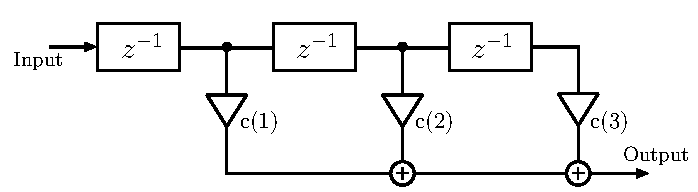
\includegraphics{fig/FIRflt.pdf}
\end{center}
\begin{center}
(b)
\end{center}

\vspace{1mm}
\setlength{\unitlength}{0.9mm}
\begin{center}
  \leavevmode
  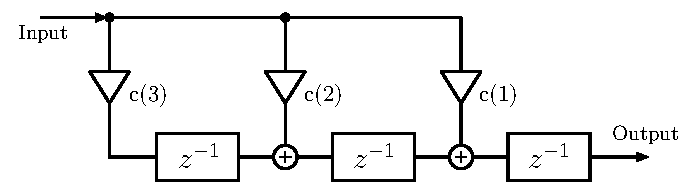
\includegraphics{fig/transflt.pdf}
\end{center}
\begin{center}
(c)
\end{center}

\vspace{1mm}
\setlength{\unitlength}{0.9mm}
\begin{center}
\begin{picture}(80,20)(10,0)
  \thicklines
  \put(15,0){\framebox(32,16){$R_L(F_1(z))$}}
  \put(57,0){\framebox(32,16){$R_L(F_2(z))$}}
  \put(0,8){\vector(1,0){15}}
  \put(47,8){\vector(1,0){10}}
  \put(89,8){\vector(1,0){15}}
  \put(0,10){\makebox(0,0)[lb]{Input}}
  \put(91,10){\makebox(0,0)[lb]{Output}}
\end{picture}
\end{center}
\begin{center}
(d)
\end{center}

\caption{\protect\parbox[t]{8cm}{
	(a)~~$R_L(F(z))\simeq D(z)$~~~$L=4$ \protect\\
	(d)~~2 level cascade realization\protect\\
        \hspace*{5mm} $R_L(F_1(z))\cdot R_L(F_2(z))\simeq D(z)$
}}
\label{fig:lmadflt_LMA}

\end{figure}

\setcounter{table}{0}
\begin{table}
        \caption{The values for the coefficients $A_{L,l}$}
        \label{tbl:lmadflt_coef}
        \setlength{\arrayrulewidth}{0.5pt}
        \renewcommand{\arraystretch}{1.2}
        \begin{center}
        \begin{tabular}{|c|c|c|} \hline
        $l$     & $A_{4,l}$			& $A_{5,l}$ \\ \hline
        1       & $4.999273\times 10^{-1}$	& $4.999391\times 10^{-1}$\\
        2       & $1.067005\times 10^{-1}$      & $1.107098\times 10^{-1}$\\
        3       & $1.170221\times 10^{-2}$      & $1.369984\times 10^{-2}$\\
        4       & $5.656279\times 10^{-4}$      & $9.564853\times 10^{-4}$\\
        5       &                               & $3.041721\times 10^{-5}$\\
      \hline
        \end{tabular}
        \end{center}
\label{tbl:lmadflt_pade}
\end{table}

\end{qsection}


\begin{options}
	\argm{m}{M}{order of cepstrum}{25}
	\argm{p}{P}{frame period}{100}
	\argm{i}{I}{interpolation period}{1}
	\argm{P}{Pa}{order of the Pad\'e approximation\\
                     $Pa$ should be $4$ or $5$}{4}
	\argm{k}{}{filtering without gain}{FALSE}
	\argm{v}{}{inverse filter}{FALSE}
	\argm{t}{}{transpose filter}{FALSE}
        \desc[1ex]{(level 2)}
        \argm{B}{B1~B2~$\ldots$~Bn}{block size of cascaded filter,\\
        	                     where $(|B1|+\ldots+|Bn|)=m$}{FALSE}
\end{options}

\begin{qsection}{EXAMPLE}
In this example, the excitation is generated from
the pitch data read in float format from {\em data.pitch},
passed through an LMA filter obtained from cepstrum file
{\em data.cep}, and the synthesized speech is written to
{\em data.syn}.
\begin{quote}
 \verb!excite < data.pitch | lmadf -m 15 data.cep > data.syn!
\end{quote} 
If one wants to divide the filter into several blocks, the -B option
can be used to specify the block size of each filter.
For example, when dividing 15-dimentional filter into 3 sub-parts(4,
5, and 6), the corresponding command line is below.
\begin{quote}
 \verb!excite < data.pitch | lmadf -m 15 -B 4 5 6 data.cep > data.syn!
\end{quote}
If the block size value assigned by the -B option is negative, the
block is not used.
\begin{quote}
 \verb!excite < data.pitch | lmadf -m 15 -B 4 -5 6 data.cep > data.syn!
\end{quote}

\end{qsection}

\begin{qsection}{NOTICE}
$Pa$ = 4 or 5.\\
\end{qsection}

\begin{qsection}{SEE ALSO}
\hyperlink{uels}{uels},
\hyperlink{acep}{acep},
\hyperlink{poledf}{poledf},
\hyperlink{ltcdf}{ltcdf},
\hyperlink{glsadf}{glsadf},
\hyperlink{mlsadf}{mlsadf},
\hyperlink{mglsadf}{mglsadf}
\end{qsection}
